\begin{figure}[ht!]  % 'htbp' option suggests placement: here, top, bottom, or on a separate page
    \centering  % Centers the TikZ picture within the figure environment
    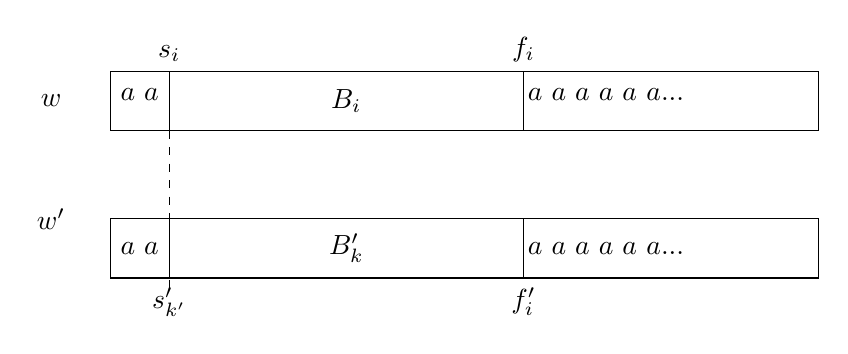
\begin{tikzpicture}[scale=1.5]
        % Draw the undivided rectangle with half height
        \draw (0.5,0) rectangle (3.5,0.5);
        \draw (0,0) rectangle (6,0.5);
        
        \node at (-0.5, 0.25) {\(w\)};
        \node at (-0.5, -0.75) {\(w'\)};
        
        \node at (2, 0.25) {\(B_i\)};
        \node[above] at (0.5,0.5) {\(s_i\)};
        \node[above] at (3.5,0.5) {\(f_i\)};

        \node at (3.6, 0.3) {\(a\)};  % Centered node in the third division
        \node at (3.8, 0.3) {\(a\)};  % Centered node in the third division
        \node at (4.0, 0.3) {\(a\)};  % Centered node in the third division
        \node at (4.2, 0.3) {\(a\)};  % Centered node in the third division
        \node at (4.4, 0.3) {\(a\)};  % Centered node in the third division
        \node at (4.7, 0.3) {\(a...\)};  % Centered node in the third division
        \node at (0.15, 0.3) {\(a\)};
        \node at (0.35, 0.3) {\(a\)};

        % Draw the divided rectangle, narrower and with half the height of the first rectangle, moved closer
        \draw (0.5,-0.75) rectangle (3.5,-1.25);  % Kept at adjusted vertical position and reduced height
        \draw (0,-0.75) rectangle (6,-1.25);

        
        \node[below] at (0.5,-1.25) {\(s'_{k'}\)};  % Label at the bottom-left corner of the second division
        \node at (2.0, -1) {\(B'_{k}\)};  % Centered node in the second division
        \node[below] at (3.5,-1.25) {\(f'_{i}\)};  % Label at the bottom between first and second division

        \node at (3.6, -1) {\(a\)};  % Centered node in the third division        
        \node at (3.8, -1) {\(a\)};  % Centered node in the third division
        \node at (4.0, -1) {\(a\)};  % Centered node in the third division
        \node at (4.2, -1) {\(a\)};  % Centered node in the third division
        \node at (4.4, -1) {\(a\)};  % Centered node in the third division
        \node at (4.7, -1) {\(a...\)};  % Centered node in the third division
        \node at (0.15, -1) {\(a\)};
        \node at (0.35, -1) {\(a\)};

        

                % Add a vertical dashed line at x = 2.5, spanning both rectangles
        \draw[dashed] (0.5, 0.0) -- (0.5, -1.35);


        
        
    \end{tikzpicture}
    \caption{$B'_{k}$ starts inside $B_i$ where $s'_{i}=s_i$ and $f'_{i}=f_i$}
    \label{fig:startinside_0}  % Label for referencing the figure in text
\end{figure}

\begin{figure}[H]  % 'htbp' option suggests placement: here, top, bottom, or on a separate page
    \centering  % Centers the TikZ picture within the figure environment
    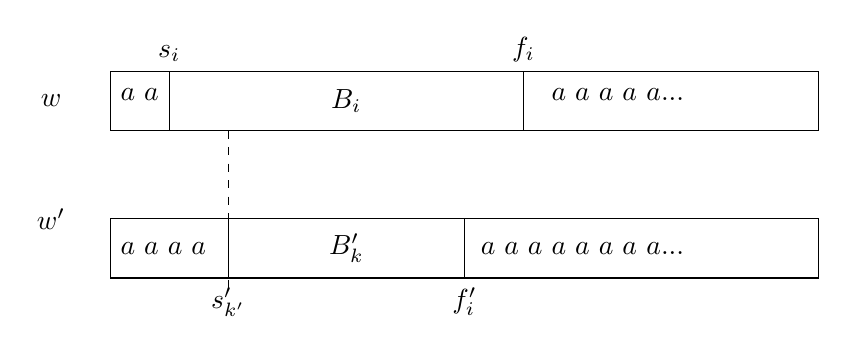
\begin{tikzpicture}[scale=1.5]
        % Draw the undivided rectangle with half height
        \draw (0.5,0) rectangle (3.5,0.5);
        \draw (0,0) rectangle (6,0.5);
        
        \node at (-0.5, 0.25) {\(w\)};
        \node at (-0.5, -0.75) {\(w'\)};
        
        \node at (2, 0.25) {\(B_i\)};
        \node[above] at (0.5,0.5) {\(s_i\)};
        \node[above] at (3.5,0.5) {\(f_i\)};
        
        \node at (3.8, 0.3) {\(a\)};  % Centered node in the third division
        \node at (4.0, 0.3) {\(a\)};  % Centered node in the third division
        \node at (4.2, 0.3) {\(a\)};  % Centered node in the third division
        \node at (4.4, 0.3) {\(a\)};  % Centered node in the third division
        \node at (4.7, 0.3) {\(a...\)};  % Centered node in the third division
        \node at (0.15, 0.3) {\(a\)};
        \node at (0.35, 0.3) {\(a\)};

        % Draw the divided rectangle, narrower and with half the height of the first rectangle, moved closer
        \draw (1,-0.75) rectangle (3.0,-1.25);  % Kept at adjusted vertical position and reduced height
        \draw (0,-0.75) rectangle (6,-1.25);

        
        \node[below] at (1.0,-1.25) {\(s'_{k'}\)};  % Label at the bottom-left corner of the second division
        \node at (2.0, -1) {\(B'_{k}\)};  % Centered node in the second division
        \node[below] at (3.0,-1.25) {\(f'_{i}\)};  % Label at the bottom between first and second division

        \node at (3.2, -1) {\(a\)};  % Centered node in the third division
        \node at (3.4, -1) {\(a\)};  % Centered node in the third division
        \node at (3.6, -1) {\(a\)};  % Centered node in the third division
        \node at (3.8, -1) {\(a\)};  % Centered node in the third division
        \node at (4.0, -1) {\(a\)};  % Centered node in the third division
        \node at (4.2, -1) {\(a\)};  % Centered node in the third division
        \node at (4.4, -1) {\(a\)};  % Centered node in the third division
        \node at (4.7, -1) {\(a...\)};  % Centered node in the third division
        \node at (0.55, -1) {\(a\)};
        \node at (0.75, -1) {\(a\)};
        
        \node at (0.15, -1) {\(a\)};
        \node at (0.35, -1) {\(a\)};

                % Add a vertical dashed line at x = 2.5, spanning both rectangles
        \draw[dashed] (1.0, 0.0) -- (1.0, -1.35);
        
        
    \end{tikzpicture}
    \caption{$B'_{k}$ starts inside $B_i$ where $f'_{i}<f_i$}
    \label{fig:startinside_a}  % Label for referencing the figure in text
\end{figure}

\begin{figure}[H]  % 'htbp' option suggests placement: here, top, bottom, or on a separate page
    \centering  % Centers the TikZ picture within the figure environment
    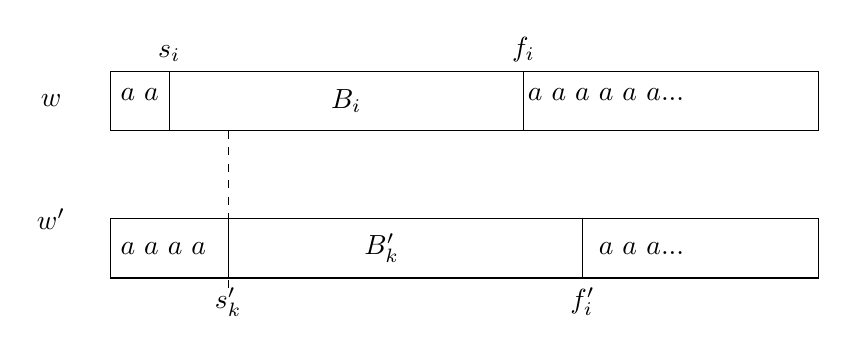
\begin{tikzpicture}[scale=1.5]
        % Draw the undivided rectangle with half height
        \draw (0.5,0) rectangle (3.5,0.5);
        \draw (0,0) rectangle (6,0.5);
        
        \node at (-0.5, 0.25) {\(w\)};
        \node at (-0.5, -0.75) {\(w'\)};
        
        \node at (2, 0.25) {\(B_i\)};
        \node[above] at (0.5,0.5) {\(s_i\)};
        \node[above] at (3.5,0.5) {\(f_i\)};
        
        \node at (3.6, 0.3) {\(a\)};  % Centered node in the third division
        \node at (3.8, 0.3) {\(a\)};  % Centered node in the third division
        \node at (4.0, 0.3) {\(a\)};  % Centered node in the third division
        \node at (4.2, 0.3) {\(a\)};  % Centered node in the third division
        \node at (4.4, 0.3) {\(a\)};  % Centered node in the third division
        \node at (4.7, 0.3) {\(a...\)};  % Centered node in the third division
        \node at (0.15, 0.3) {\(a\)};
        \node at (0.35, 0.3) {\(a\)};

        % Draw the divided rectangle, narrower and with half the height of the first rectangle, moved closer
        \draw (1,-0.75) rectangle (4.0,-1.25);  % Kept at adjusted vertical position and reduced height
        \draw (0,-0.75) rectangle (6,-1.25);

        
        \node[below] at (1.0,-1.25) {\(s'_{k}\)};  % Label at the bottom-left corner of the second division
        \node at (2.3, -1) {\(B'_{k}\)};  % Centered node in the second division
        \node[below] at (4.0,-1.25) {\(f'_{i}\)};  % Label at the bottom between first and second division

        
        
        \node at (4.2, -1) {\(a\)};  % Centered node in the third division
        \node at (4.4, -1) {\(a\)};  % Centered node in the third division
        \node at (4.7, -1) {\(a...\)};  % Centered node in the third division
        \node at (0.15, -1) {\(a\)};
        \node at (0.35, -1) {\(a\)};
        \node at (0.55, -1) {\(a\)};
        \node at (0.75, -1) {\(a\)};
        
        \draw[dashed] (1.0, 0.0) -- (1.0, -1.35);
        
        
        
    \end{tikzpicture}
    \caption{$B'_{k}$ starts inside $B_i$ where $s_i\leq s'_k \leq f_i$}
    \label{fig:startinside_b}  % Label for referencing the figure in text
\end{figure}
